% Generated by make_results_figures.py from media/data/*.json.
% Those numbers are DIGITIZED from the published figures, not the
% original data: see media/data/README.md.
\documentclass[border=6pt]{standalone}
\usepackage[T1]{fontenc}
\usepackage{helvet}
\renewcommand{\familydefault}{\sfdefault}
\usepackage{amsmath}
\usepackage{tikz}
\usetikzlibrary{arrows.meta,calc,decorations.pathreplacing}
\definecolor{spaceC}{HTML}{3B6EA5}
\definecolor{timeC}{HTML}{D9822B}
\definecolor{hcC}{HTML}{6B5B95}
\definecolor{vcC}{HTML}{8A7F72}
\definecolor{ink}{HTML}{2B2B2B}
\definecolor{muted}{HTML}{6B6B6B}
\definecolor{gridC}{HTML}{E6E4E0}
\definecolor{nanC}{HTML}{EFEDEA}
\definecolor{s1}{HTML}{2A78D6}
\definecolor{s2}{HTML}{EB6834}
\definecolor{s3}{HTML}{1BAF7A}
\definecolor{s4}{HTML}{EDA100}
\definecolor{s5}{HTML}{E87BA4}
\begin{document}
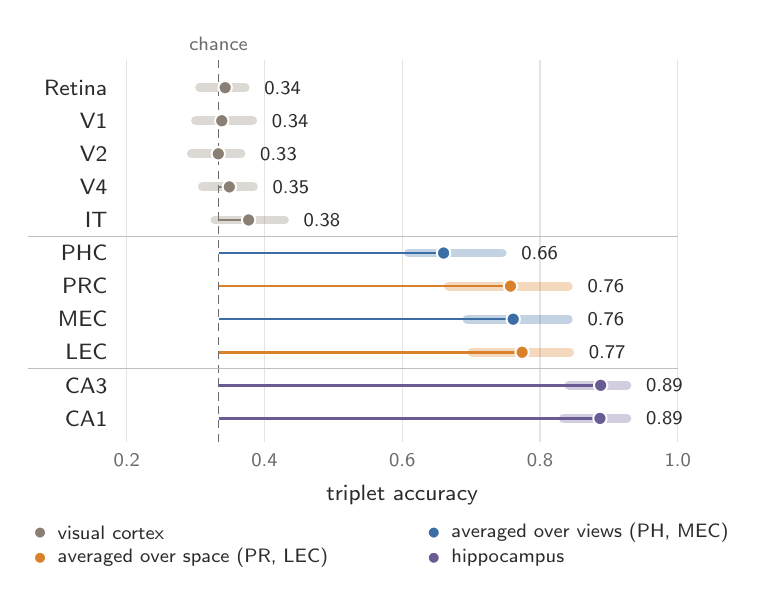
\begin{tikzpicture}[font=\footnotesize,
  tick/.style={font=\scriptsize,text=muted},
  lab/.style={font=\footnotesize,text=ink},
  ttl/.style={font=\small\bfseries,anchor=west,text=ink}]

\draw[gridC,line width=0.4pt] (0.000,-0.3)--(0.000,4.550);
\node[tick,anchor=north] at (0.000,-0.32) {0.2};
\draw[gridC,line width=0.4pt] (1.750,-0.3)--(1.750,4.550);
\node[tick,anchor=north] at (1.750,-0.32) {0.4};
\draw[gridC,line width=0.4pt] (3.500,-0.3)--(3.500,4.550);
\node[tick,anchor=north] at (3.500,-0.32) {0.6};
\draw[gridC,line width=0.4pt] (5.250,-0.3)--(5.250,4.550);
\node[tick,anchor=north] at (5.250,-0.32) {0.8};
\draw[gridC,line width=0.4pt] (7.000,-0.3)--(7.000,4.550);
\node[tick,anchor=north] at (7.000,-0.32) {1.0};
\node[lab,anchor=north] at (3.500,-0.72) {triplet accuracy};
\draw[muted,densely dashed,line width=0.5pt] (1.167,-0.3)--(1.167,4.550);
\node[tick,anchor=south] at (1.167,4.550) {chance};
\draw[black!25,line width=0.4pt] (-1.25,2.310)--(7.000,2.310);
\draw[black!25,line width=0.4pt] (-1.25,0.630)--(7.000,0.630);
\draw[vcC,line width=0.9pt] (1.167,4.200)--(1.251,4.200);
\draw[vcC,line width=3.2pt,opacity=0.3,line cap=round] (0.927,4.200)--(1.505,4.200);
\filldraw[fill=vcC,draw=white,line width=0.7pt] (1.251,4.200) circle (0.085);
\node[lab,anchor=east] at (-0.12,4.200) {Retina};
\node[tick,text=ink,anchor=west] at (1.625,4.200) {0.34};
\draw[vcC,line width=0.9pt] (1.167,3.780)--(1.208,3.780);
\draw[vcC,line width=3.2pt,opacity=0.3,line cap=round] (0.875,3.780)--(1.601,3.780);
\filldraw[fill=vcC,draw=white,line width=0.7pt] (1.208,3.780) circle (0.085);
\node[lab,anchor=east] at (-0.12,3.780) {V1};
\node[tick,text=ink,anchor=west] at (1.721,3.780) {0.34};
\draw[vcC,line width=0.9pt] (1.167,3.360)--(1.164,3.360);
\draw[vcC,line width=3.2pt,opacity=0.3,line cap=round] (0.822,3.360)--(1.452,3.360);
\filldraw[fill=vcC,draw=white,line width=0.7pt] (1.164,3.360) circle (0.085);
\node[lab,anchor=east] at (-0.12,3.360) {V2};
\node[tick,text=ink,anchor=west] at (1.572,3.360) {0.33};
\draw[vcC,line width=0.9pt] (1.167,2.940)--(1.304,2.940);
\draw[vcC,line width=3.2pt,opacity=0.3,line cap=round] (0.962,2.940)--(1.610,2.940);
\filldraw[fill=vcC,draw=white,line width=0.7pt] (1.304,2.940) circle (0.085);
\node[lab,anchor=east] at (-0.12,2.940) {V4};
\node[tick,text=ink,anchor=west] at (1.730,2.940) {0.35};
\draw[vcC,line width=0.9pt] (1.167,2.520)--(1.549,2.520);
\draw[vcC,line width=3.2pt,opacity=0.3,line cap=round] (1.120,2.520)--(2.004,2.520);
\filldraw[fill=vcC,draw=white,line width=0.7pt] (1.549,2.520) circle (0.085);
\node[lab,anchor=east] at (-0.12,2.520) {IT};
\node[tick,text=ink,anchor=west] at (2.124,2.520) {0.38};
\draw[spaceC,line width=0.9pt] (1.167,2.100)--(4.025,2.100);
\draw[spaceC,line width=3.2pt,opacity=0.3,line cap=round] (3.579,2.100)--(4.769,2.100);
\filldraw[fill=spaceC,draw=white,line width=0.7pt] (4.025,2.100) circle (0.085);
\node[lab,anchor=east] at (-0.12,2.100) {PHC};
\node[tick,text=ink,anchor=west] at (4.889,2.100) {0.66};
\draw[timeC,line width=0.9pt] (1.167,1.680)--(4.874,1.680);
\draw[timeC,line width=3.2pt,opacity=0.3,line cap=round] (4.086,1.680)--(5.609,1.680);
\filldraw[fill=timeC,draw=white,line width=0.7pt] (4.874,1.680) circle (0.085);
\node[lab,anchor=east] at (-0.12,1.680) {PRC};
\node[tick,text=ink,anchor=west] at (5.729,1.680) {0.76};
\draw[spaceC,line width=0.9pt] (1.167,1.260)--(4.909,1.260);
\draw[spaceC,line width=3.2pt,opacity=0.3,line cap=round] (4.322,1.260)--(5.609,1.260);
\filldraw[fill=spaceC,draw=white,line width=0.7pt] (4.909,1.260) circle (0.085);
\node[lab,anchor=east] at (-0.12,1.260) {MEC};
\node[tick,text=ink,anchor=west] at (5.729,1.260) {0.76};
\draw[timeC,line width=0.9pt] (1.167,0.840)--(5.022,0.840);
\draw[timeC,line width=3.2pt,opacity=0.3,line cap=round] (4.384,0.840)--(5.626,0.840);
\filldraw[fill=timeC,draw=white,line width=0.7pt] (5.022,0.840) circle (0.085);
\node[lab,anchor=east] at (-0.12,0.840) {LEC};
\node[tick,text=ink,anchor=west] at (5.746,0.840) {0.77};
\draw[hcC,line width=0.9pt] (1.167,0.420)--(6.020,0.420);
\draw[hcC,line width=3.2pt,opacity=0.3,line cap=round] (5.617,0.420)--(6.353,0.420);
\filldraw[fill=hcC,draw=white,line width=0.7pt] (6.020,0.420) circle (0.085);
\node[lab,anchor=east] at (-0.12,0.420) {CA3};
\node[tick,text=ink,anchor=west] at (6.473,0.420) {0.89};
\draw[hcC,line width=0.9pt] (1.167,0.000)--(6.011,0.000);
\draw[hcC,line width=3.2pt,opacity=0.3,line cap=round] (5.547,0.000)--(6.353,0.000);
\filldraw[fill=hcC,draw=white,line width=0.7pt] (6.011,0.000) circle (0.085);
\node[lab,anchor=east] at (-0.12,0.000) {CA1};
\node[tick,text=ink,anchor=west] at (6.473,0.000) {0.89};
\filldraw[fill=vcC,draw=white,line width=0.6pt] (-1.100,-1.450) circle (0.075);
\node[tick,text=ink,anchor=west] at (-1.000,-1.450) {visual cortex};
\filldraw[fill=spaceC,draw=white,line width=0.6pt] (3.900,-1.450) circle (0.075);
\node[tick,text=ink,anchor=west] at (4.000,-1.450) {averaged over views (PH, MEC)};
\filldraw[fill=timeC,draw=white,line width=0.6pt] (-1.100,-1.770) circle (0.075);
\node[tick,text=ink,anchor=west] at (-1.000,-1.770) {averaged over space (PR, LEC)};
\filldraw[fill=hcC,draw=white,line width=0.6pt] (3.900,-1.770) circle (0.075);
\node[tick,text=ink,anchor=west] at (4.000,-1.770) {hippocampus};
\end{tikzpicture}
\end{document}

